\section{Lead Glass Shower Counters}
  
% This section written by P. Markowitz in Novermber 1996.
% V1.0 - OSP for PbG shower counters use
% Direct all comments/questions to:
% markowit@cebaf.gov
% TJNAF Room 16-116
% (757) 249 7237
% Updated:  April-18-1999 pecm included Armen's descriptions from web

\subsection{Overview}

Electromagnetic shower counters offer a useful means of particle
identification (PID) \cite{bartozek}-\cite{appel}. Shower counters
complement other means of PID such as time-of-flight (TOF) or
threshold Cerenkov counters, due to the independent physical processes
responsible which result in different detector
limitations \cite{goldberg}. Independent PID allows multiple detectors
($i.e.$, a Cerenkov counter followed by a shower counter) to obtain
excellent rejection ratios that are the product of the individual
rejection ratios.

Shower counters measure the energy deposited by the incoming particle.  
The detected light output is linearly proportional to the energy lost
by the incoming particle.  Electromagnetic showers are stopped in the 
counters, whereas hadronic showers, due to the longer hadronic mean free 
path, are not.  Looking at the longitudinal distribution of the energy 
deposited in the calorimeter differentiates between electromagnetic and 
hadronic showers and therefore identifies the incident particle.

Typical pion rejection with a lead glass counter is of the order of 
100-1000:1 in the 1 to 10 GeV region \cite{ferbel}.
The Hall A electromagnetic shower counter is meant to offer rejection 
ratios better than 100:1 \cite{CDR}.  
The limitation in using a shower counter comes from separating the tails
of the distributions, and is therefore dependent on energy resolution.
At higher energy the relative resolution of a shower counter improves, leading
to better separation between distributions.  Conversely, other techniques
perform worse at higher energy.  
The TOF separation for a given path length decreases, and above 4 GeV/c pions
can trigger a threshold CO$_2$ Cerenkov counter operated at standard 
temperature and pressure (STP) \cite{ferbel}. 
[The threshold for a CO$_2$ Cerenkov counter at STP is $\gamma=34.1$, meaning 
that for an electron the threshold is just over 17 MeV, while for a pion the
threshold is just over 4 GeV/c momentum].

A Cerenkov counter is routinely capable of pion rejection 
of the order of 1000:1 at CEBAF energies \cite{ferbel}.  A combination of
successive Cerenkov counters might achieve higher rejection ratios.  
However this only works if the backgrounds in the two devices are 
uncorrelated.  A knock-on electron which triggers 
the first Cerenkov counter and travels forward through both detectors 
will also trigger the second.  Independent PID provided by a measurement 
of the particle energy in a shower counter offers a solution to this 
problem of correlated backgrounds.  Used in conjunction with a threshold 
Cerenkov counter, the combination can achieve rejection ratios of 
$5\times 10^5$ \cite{CDR}.

The Hall A electron spectrometer is equipped with a 2-layer, segmented
shower counter.  The first layer, the so-called ``pre-shower'' counter
is made of 48 blocks of TF1 lead glass.  Each block is nominally
10 cm by
10 cm by 35 cm long.  The second layer, the so-called ``total absorber'' 
counter is nominally 15 cm by 15 cm by 35 cm viewed head-on by the beam.

Operation of the shower counter requires the application of High Voltage
(HV) across the photomultiplier tubes and bases, which are mounted on the
back of the shower counter blocks for the total absorber and on the sides 
of the shower counter in the case of the pre-shower, within the confines of 
the protective aluminum support frame.

As charged particles pass through the lead glass of the shower counter, they
produce electron-positron particle-antiparticle pairs.  These particles in 
turn both produce additional particles and Cerenkov light which is collected 
in the phototubes.  The pulses are then amplified, delayed and sent to
ADCs, which are gated by the overall event trigger.  The ADCs are read out 
by the {\it CODA} acquisition software.  The data are histogrammed online by 
the {\it DHIST} software.  In-depth offline data analysis requires the 
{\it ESPACE} software.

\subsection{Operating Procedures}

\paragraph{Power Supplies and Electronics Procedures}

The HV power supplies and readout electronics associated with the HRS
VDCs are all commercially designed.  The reader is directed towards
the manuals made available by the manufacturer for the detailed
information not provided here.

The LeCroy HV power supply provides -1500 V nominal to
the total absorber and 1200 V to the preshower.
The power supply is located in
the detector hut in a NIM bin on the upper level of the space frame.
This unit may be controlled either manually or remotely via the
{\it EPICS} control software, and also provides a monitor of the
current drawn by each phototube to which it is attached.
Connections from the power supply to the base are made using
standard SHV connectors mounted on red RG-59/U HV cable good to 5 kV.
Typical values of the high voltages are shown in the tables for both the 
pre-radiator and the total absorber.

If at all possible, the HV and LV power supplies should be left
on continuously.   This allows the tube noise to quiet down after high
voltage is applied and the temperature of the base components stabilizes.

%\vfill\eject
\begin{figure}
\begin{center}
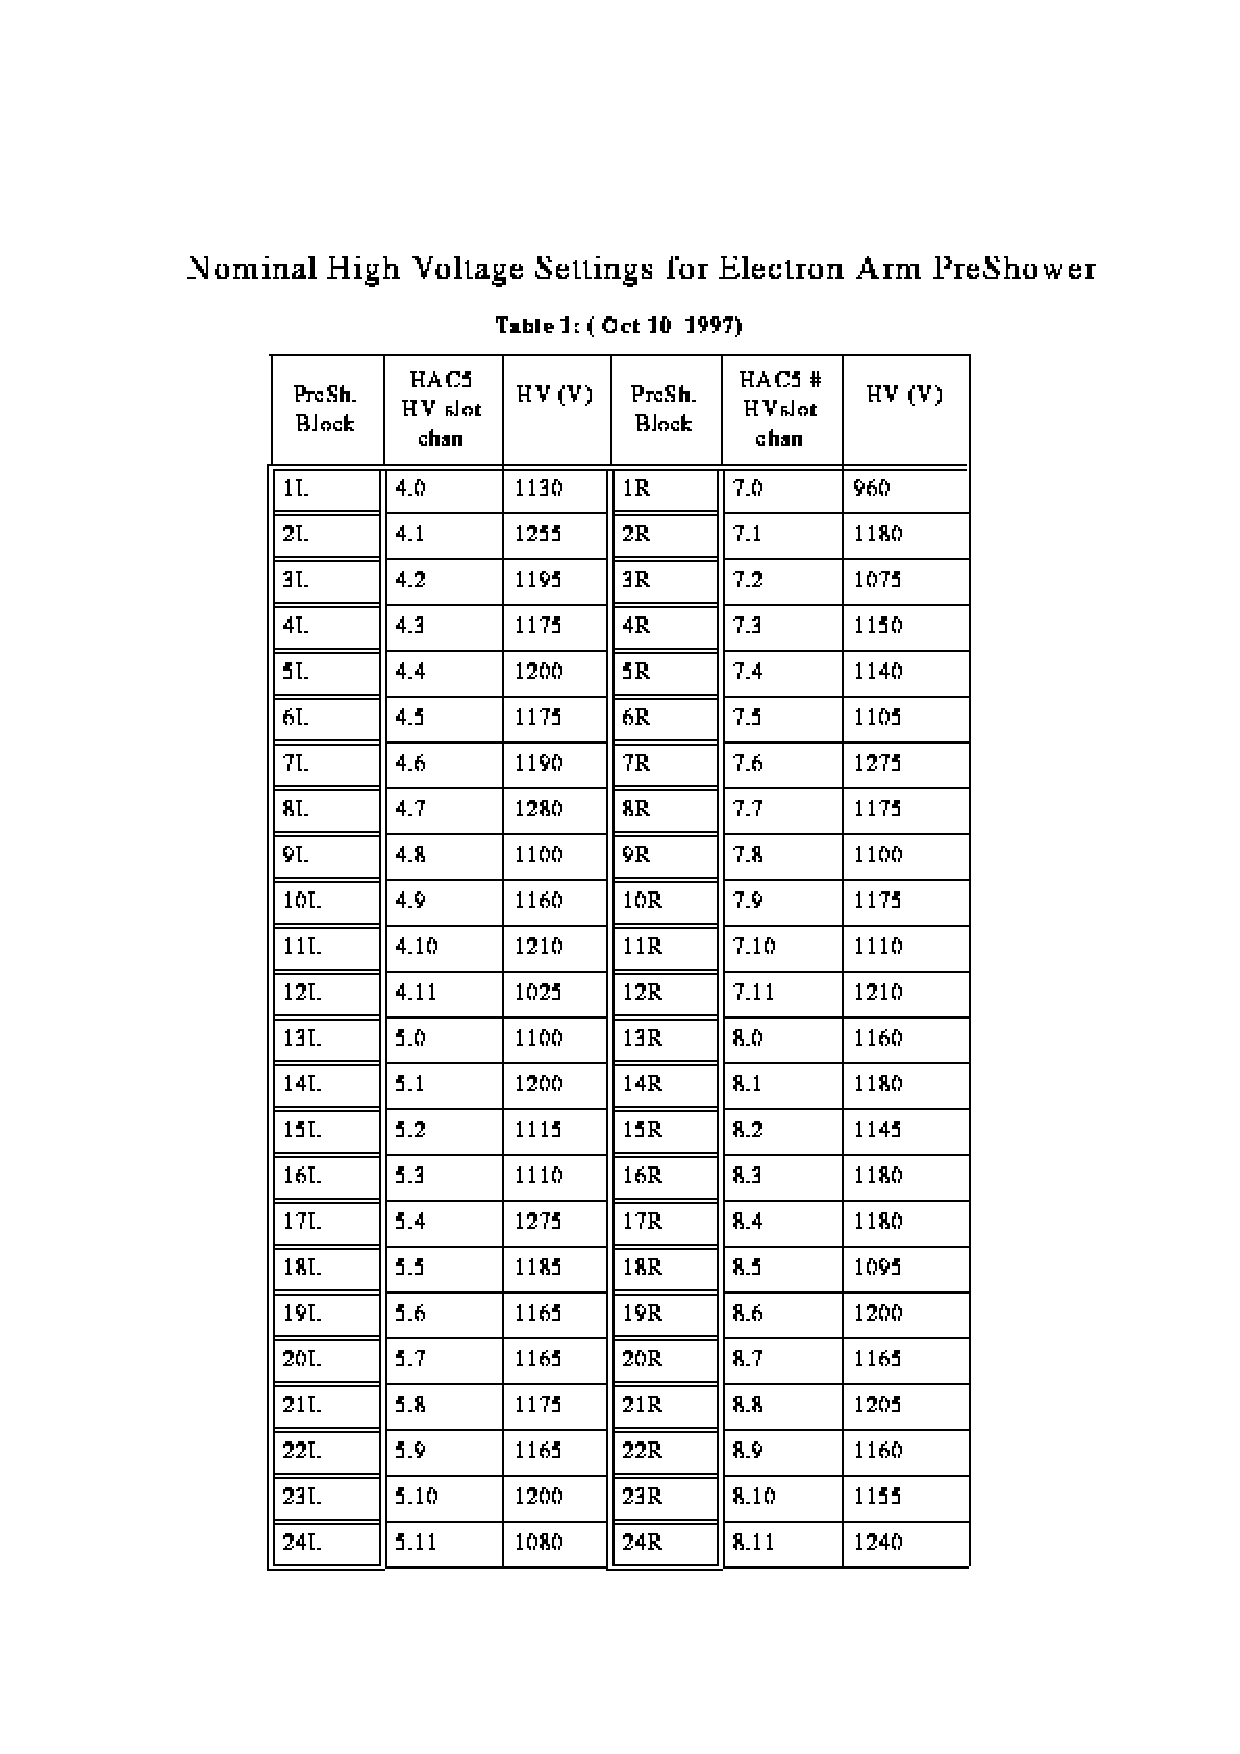
\includegraphics[angle=0,width=15cm,clip]{pshHV}
{\linespread{1.}
\caption[Detectors: Pre-shower Counter HV]
{Typical values of the preshower counter high voltages.}
\label{fig:pre_hv}}
\end{center}
\end{figure}

\begin{figure}
\begin{center}
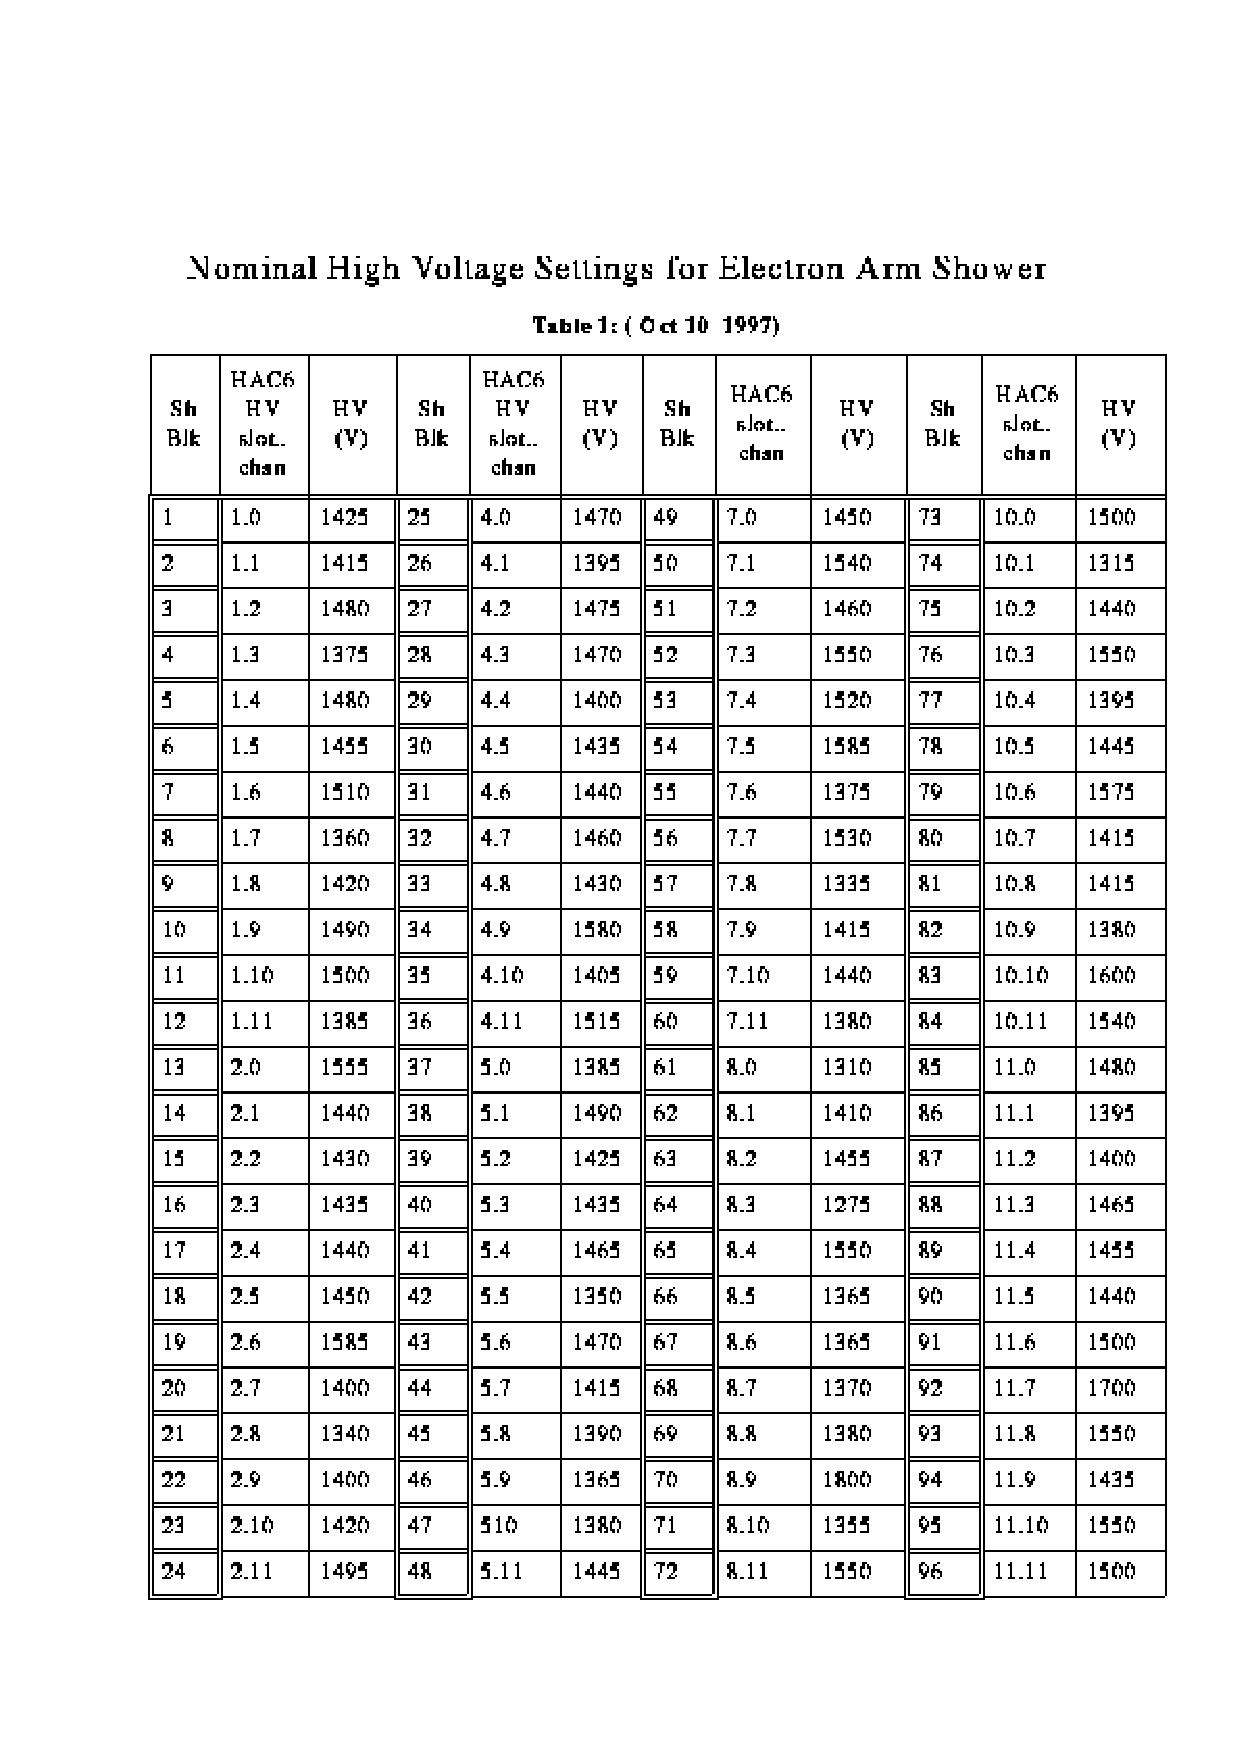
\includegraphics[angle=0,width=15cm,clip]{shHV}
{\linespread{1.}
\caption[Detectors: Shower Counter HV]{Typical values of the
total absorption counterhigh voltages.}
\label{fig:ta_hv}}
\end{center}
\end{figure}

\paragraph{Signal Handling, Summing, Amplification and the Multiplexer}

The upstairs electronics racks hold two NIM bins containing the summing modules
of the multiplexer.  The output of these is sent to the ADCs.  Both the 
individual channels and the sum of every six channels is sent into an ADC 
where it can later be analyzed by the software.  The operations manual for 
the multiplexer was written by H. Breuer (UMd) and is available from him upon 
request.

The detector signals are physically plugged into the ADC channels
 and connected to the signal wires labelled as shown in the
 diagrams below,
 for both the preshower counter and the total absorber counter.
 
\begin{figure}
\begin{center}
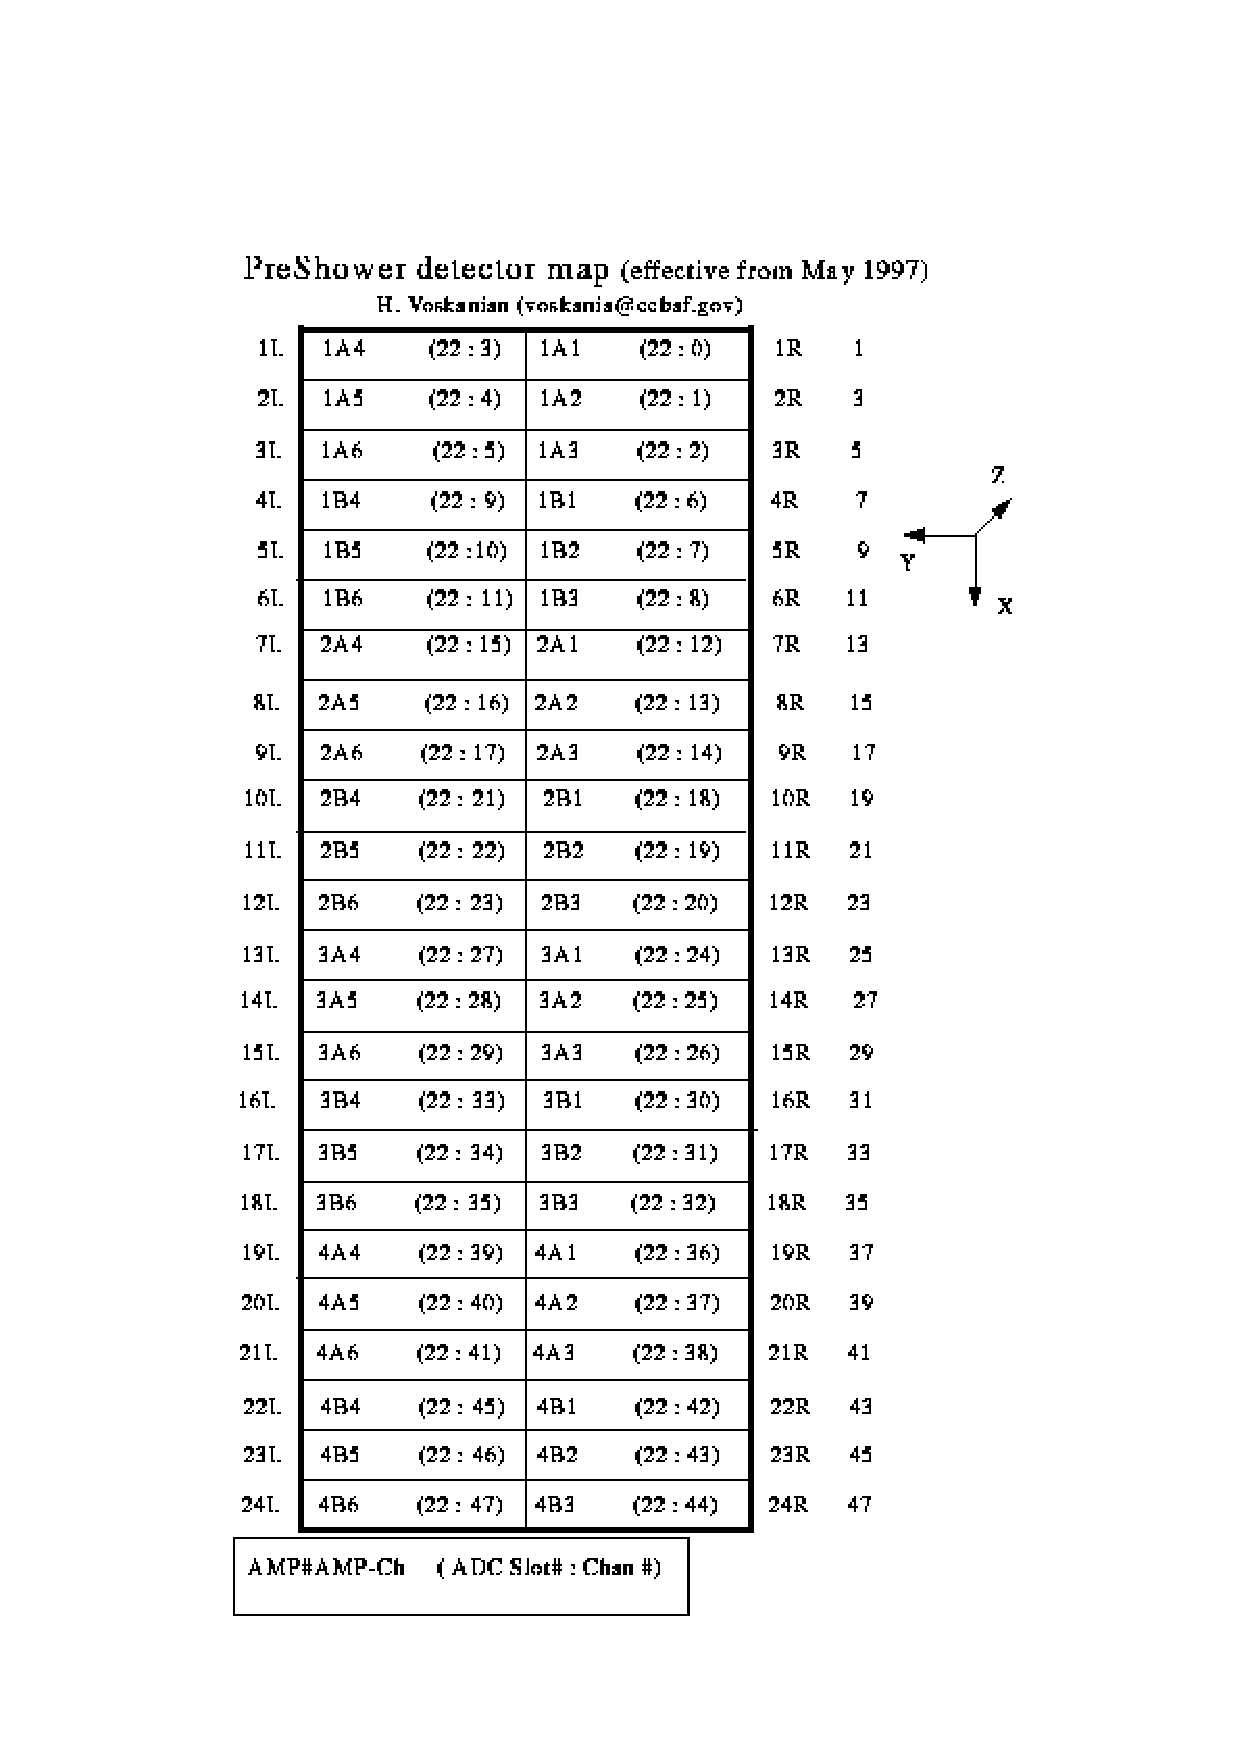
\includegraphics[angle=0,width=15cm,clip]{PreSh_det_map}
{\linespread{1.}
\caption[Detectors: Map of Pre-shower detector]{Map of the Pre-shower counter detectors.}
\label{fig:pre_map_}}
\end{center}
\end{figure}

\begin{figure}
\begin{center}
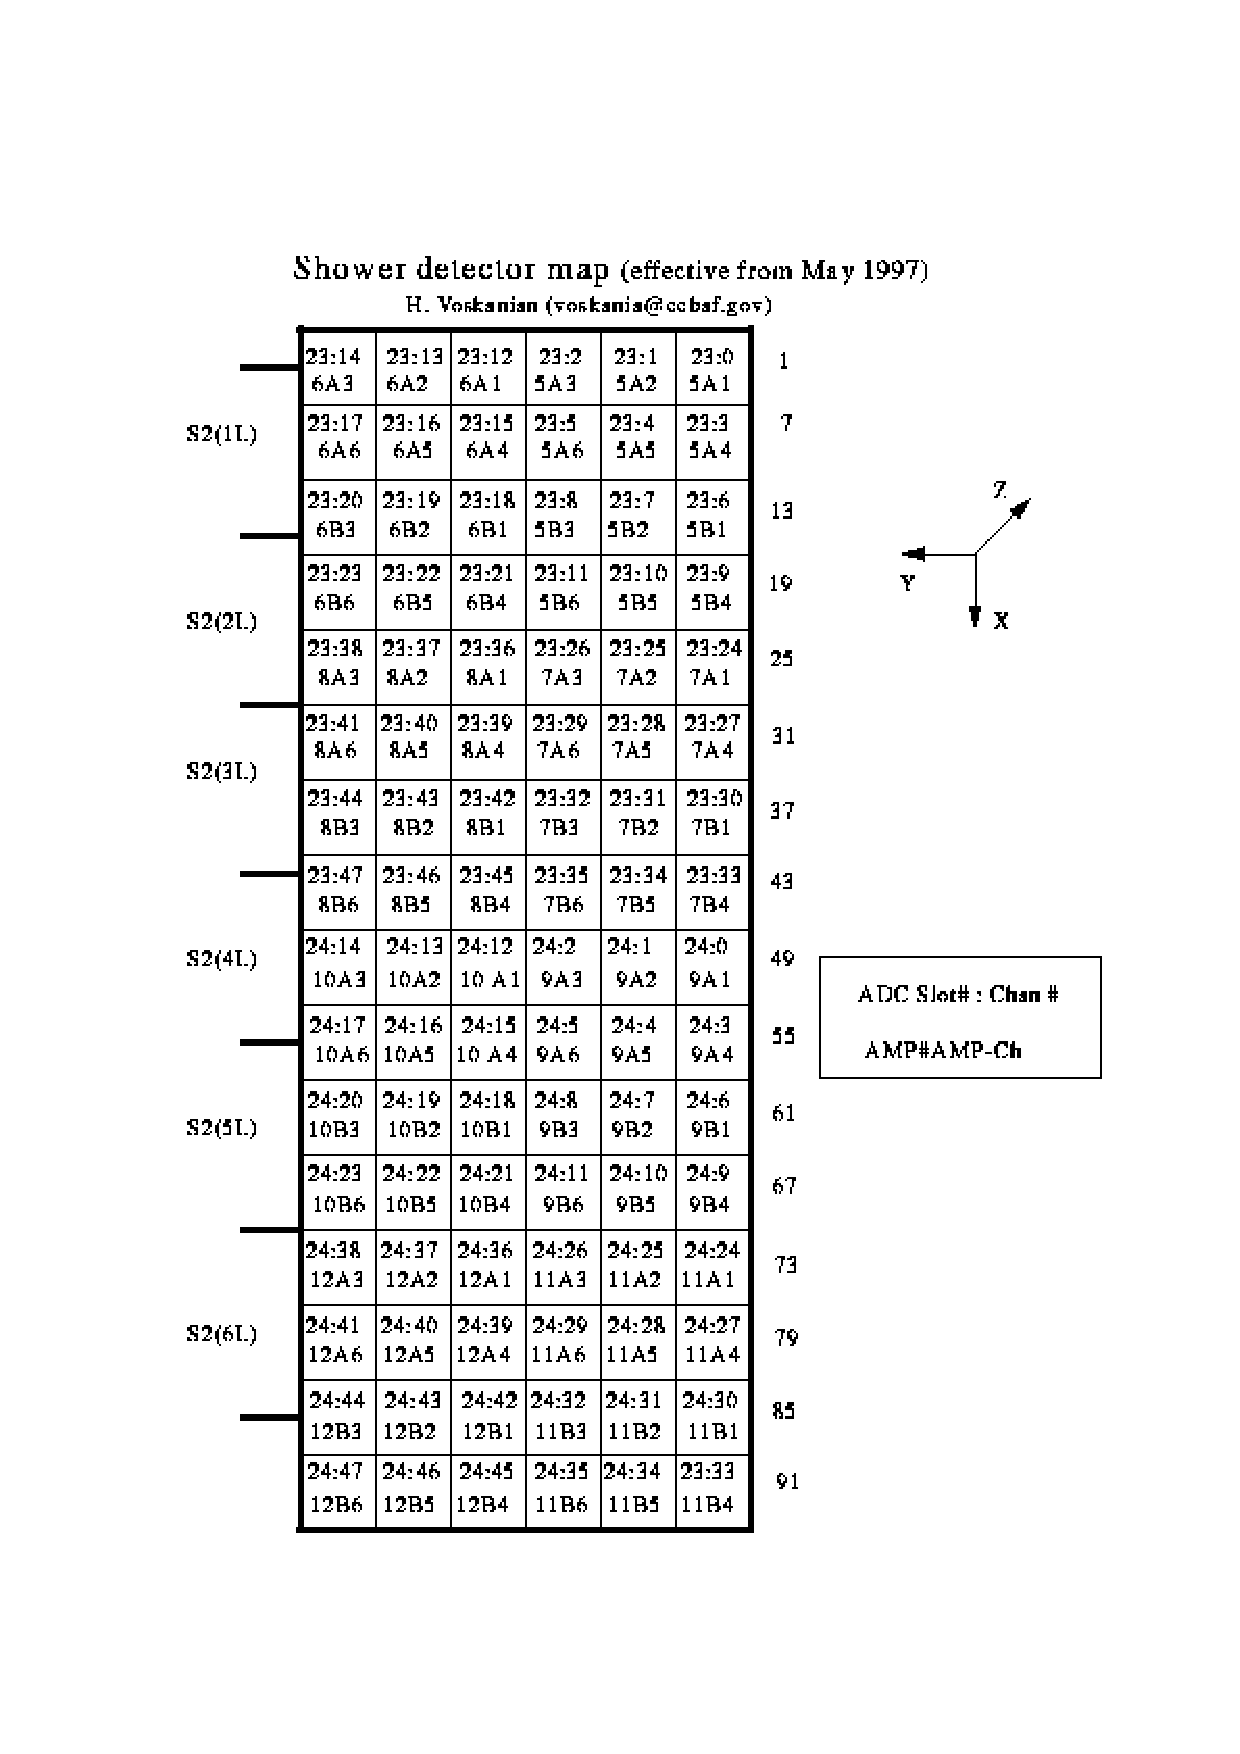
\includegraphics[angle=0,width=15cm,clip]{Shwr_det_map}
{\linespread{1.}
\caption[Detectors: Map of shower detector]{Map of the shower counter detectors.}
\label{fig:ta_map}}
\end{center}
\end{figure}

\subsection{Handling Considerations}

The shower counters are very delicate devices which are easily damaged.
Thus, care must be exercised whenever they are moved or used.

\begin{itemize}
\item{Before turning on the high voltage for the shower counters (HAC5 for the preshower 
and HAC6 for the total absorber), check the shower counter log book located in the Hall 
A counting house for the latest values of the high voltage.}

\item{Never disconnect or connect all the high voltage to the bases with the
high voltage power turned on.  Doing so will damage the bases (the zener diodes
are destroyed).}

\item{Never service the lead glass with the high voltage on.  The
high voltage poses a safety hazard.}

\item{Never drop anything onto the bases and tubes; they are extremely fragile.  
They should not be used as support or to hold any weight.  Also, do not drop
the lead glass blocks.  They will be damaged or
destroyed.}

\item{When ramping the HV, keep an eye on the current drawn by the
individual bases.  A light leak in the wrapping will produce a large current
( $ > 1 \mu$A at low voltages (1 kV).  If the tubes draw an excess amount of current
turn them off and check for leaks in the wrapping.}
\end{itemize}


\subsection{Safety Assessment}
The following potential hazards have been clearly identified.
\begin{description}
\item {\bf The High Voltage System} The LeCroy 1443 HV crate equipped
with LeCroy 1461N negative high voltage cards supplies provides
up to 3.3 kV of low current power.  Red HV RG-59/U cable good to 5 kV with
standard SHV connectors is used to connect the power supply to the
photomultiplier tube voltage divider bases.  A given base on the TA
draws typically 500-600 $\mu A$ of current with the high voltage
on at between 1400 and 1500 V.  The PS bases typically draw 900 $\mu A$
with the high voltage on at between 1100 and 1200 V.

\item {\bf The Lead Glass Support Structure}
The lead glass shower counters are mounted on top of the space
frame for the detectors.  Access for servicing the shower counters
requires climbing on top of the support frame.  Only the responsible
personnel identified below should attempt to service the shower counter;
such work requires proper safety precautions and prior training/experience.

\item {\bf The Lead Glass blocks}
The lead glass shower blocks and tubes weigh approximately 70 -- 80 pounds
apiece.  Lifting, replacing, or moving such blocks should
be done properly to avoid muscle problems and damage to the blocks.

\end{description}

\subsection{Authorized Personnel} 
The following individuals are authorized to work on shower counters. 
\begin{itemize} 
\item[~]Breuer, Herbert - 301-405-6108 
\item[~]Markowitz, Pete - x7237, 305-348-1710
\item[~]Segal, Jack - x7242 
\item[~]Voskanyan, Hakob - x5105
\item[~]Wojtsekhowski, Bogdan - x7191 
\end{itemize} 

\subsection{Software Algorithms}

The purpose of the shower cluster reconstruction in the Preshower and 
the Shower detector is to:
\begin{list}{$\bullet$}{}
\item Define all clusters of fired blocks, which belong to the showers, 
      registered in the detector;
\item Calculate parameters of showers in the detector: energy deposition of 
      showers, $X$ and $Y$ coordinates of the shower center;
\item Set parameters and identifier of the so-called ``main'' cluster.
\end{list}

\noindent Cluster in the shower detector is determined as follows:
\begin{list}{---}{}
\item Cluster is a group of continuous blocks; 
\item Cluster can occupy a maximum of 6 ($2 \times 3$) blocks in the case of 
      Preshower and 9 ($3 \times 3$) blocks in the case of Shower; 
\item Central block is defined as the block that has maximum energy deposition.
\end{list}

The ``main'' cluster in Preshower/Shower is the cluster with the biggest 
energy, which is coincident with the ``golden track'', or coincident with some 
Shower/Preshower cluster.
Coincidence of the cluster with the ``golden track'' means that the
distance between the
shower cluster center and crossing point of ``golden track'' with
the detector plane is less than a certain magnitude.
Coincidence of the Preshower and Shower clusters means,
that distance between the 
clusters centers is less than a certain magnitude (it is  assumed that both of
these points are on the same $Z$--plane).

The shower clusters reconstruction in Preshower and Shower is performed by the 
following steps:
\begin{enumerate}
\item Sort fired blocks in order of decreasing deposited energy; 
\item Pick out the block with maximum energy deposition and all fired blocks in
      its arrangement ($2 \times 3$ blocks for Preshower, $3 \times 3$ blocks 
      for Shower), as belonging to one cluster;
\item Remove all blocks associated with the found cluster from further 
      consideration;
\item Repeat steps 2 and 3, until all of the fired blocks are associated with 
      a cluster;
\item Calculate energy deposition, $X$ and $Y$ coordinates of each cluster and 
      sort clusters by decreasing energy deposit;
\item Define coordinates of crossing point of ``golden track'' with detector 
      plane in detector local coordinate system;
\item Analyze geometrical position of the ``golden track'' point on the 
      detector plane and cluster centers in order to determine the ``main'' 
      cluster and to set its parameters and identifier.
\end{enumerate}

Energy deposition $E$, $X$ and $Y$ coordinates of the shower center are 
calculated by the formulas: 
$$E=\sum_{i \in M}e_i\ ,\ \ \ \ 
X=\sum_{i \in M}e_i \cdot x_i/E\ ,\ \ \ \ Y=\sum_{i \in M}e_i \cdot y_i/E\ ,$$
where: $i$ --- number of detector block, included in the cluster; $M$ --- set
of blocks numbers, included in the cluster; $e_i$ --- energy deposition in 
block $i$ of detector; $x_i$, $y_i$ --- $X$ and $Y$ coordinates of center 
of block $i$ of detector.

The shower cluster reconstruction algorithm described above has been 
implemented  by the ESPACE analysis subroutine {\bf tot\_shower}.  A complete 
description of the program as well as information about the ESPACE routines 
and kumac files 
used to perform the analysis, photographs of the detectors and more 
information can be found at the URL 
\htmladdnormallinkfoot{}{\url{
http://www.jlab.org/~armen/sh_web_page/welcome.html
}}
\obsolete{
\begin{thebibliography}{99}
\bibitem{bartozek} G. Bartozek et al., NIM A301 (1991)   47-60, 
``The E760 Lead-glass Calorimeter: Design and Initial Test Results''
\bibitem{appel}    J.A. Appel  et al., NIM 127 (1975)  495-505, 
"Performance of a Lead-glass Electromagnetic Shower Detector at Fermilab" 
\bibitem{goldberg}     M. Goldberg et al., NIM 108  (1975)
119-123, "Radiation Induced Coloring of Cerenkov Coutner Glasses"
\bibitem{ferbel} ``Experimental Techniques in High-Energy Nuclear and Particle
Physics'', T. Ferbel ed., 1991.
\bibitem{CDR}  ``CEBAF Conceptual Design Report (CDR)'', 1990.
\end{thebibliography}
}

% ===========  CVS info
% $Header: /group/halla/analysis/cvs/tex/osp/src/hrs_det/shower.tex,v 1.1 2003/06/05 17:28:30 gen Exp $
% $Id: shower.tex,v 1.1 2003/06/05 17:28:30 gen Exp $
% $Author: gen $
% $Date: 2003/06/05 17:28:30 $
% $Name:  $
% $Locker:  $
% $Log: shower.tex,v $
% Revision 1.1  2003/06/05 17:28:30  gen
% Initial revision
%
